% Options for packages loaded elsewhere
\PassOptionsToPackage{unicode}{hyperref}
\PassOptionsToPackage{hyphens}{url}
%
\documentclass[
]{article}
\usepackage{amsmath,amssymb}
\usepackage{lmodern}
\usepackage{iftex}
\ifPDFTeX
  \usepackage[T1]{fontenc}
  \usepackage[utf8]{inputenc}
  \usepackage{textcomp} % provide euro and other symbols
\else % if luatex or xetex
  \usepackage{unicode-math}
  \defaultfontfeatures{Scale=MatchLowercase}
  \defaultfontfeatures[\rmfamily]{Ligatures=TeX,Scale=1}
\fi
% Use upquote if available, for straight quotes in verbatim environments
\IfFileExists{upquote.sty}{\usepackage{upquote}}{}
\IfFileExists{microtype.sty}{% use microtype if available
  \usepackage[]{microtype}
  \UseMicrotypeSet[protrusion]{basicmath} % disable protrusion for tt fonts
}{}
\makeatletter
\@ifundefined{KOMAClassName}{% if non-KOMA class
  \IfFileExists{parskip.sty}{%
    \usepackage{parskip}
  }{% else
    \setlength{\parindent}{0pt}
    \setlength{\parskip}{6pt plus 2pt minus 1pt}}
}{% if KOMA class
  \KOMAoptions{parskip=half}}
\makeatother
\usepackage{xcolor}
\usepackage[margin=1in]{geometry}
\usepackage{graphicx}
\makeatletter
\def\maxwidth{\ifdim\Gin@nat@width>\linewidth\linewidth\else\Gin@nat@width\fi}
\def\maxheight{\ifdim\Gin@nat@height>\textheight\textheight\else\Gin@nat@height\fi}
\makeatother
% Scale images if necessary, so that they will not overflow the page
% margins by default, and it is still possible to overwrite the defaults
% using explicit options in \includegraphics[width, height, ...]{}
\setkeys{Gin}{width=\maxwidth,height=\maxheight,keepaspectratio}
% Set default figure placement to htbp
\makeatletter
\def\fps@figure{htbp}
\makeatother
\setlength{\emergencystretch}{3em} % prevent overfull lines
\providecommand{\tightlist}{%
  \setlength{\itemsep}{0pt}\setlength{\parskip}{0pt}}
\setcounter{secnumdepth}{-\maxdimen} % remove section numbering
\newlength{\cslhangindent}
\setlength{\cslhangindent}{1.5em}
\newlength{\csllabelwidth}
\setlength{\csllabelwidth}{3em}
\newlength{\cslentryspacingunit} % times entry-spacing
\setlength{\cslentryspacingunit}{\parskip}
\newenvironment{CSLReferences}[2] % #1 hanging-ident, #2 entry spacing
 {% don't indent paragraphs
  \setlength{\parindent}{0pt}
  % turn on hanging indent if param 1 is 1
  \ifodd #1
  \let\oldpar\par
  \def\par{\hangindent=\cslhangindent\oldpar}
  \fi
  % set entry spacing
  \setlength{\parskip}{#2\cslentryspacingunit}
 }%
 {}
\usepackage{calc}
\newcommand{\CSLBlock}[1]{#1\hfill\break}
\newcommand{\CSLLeftMargin}[1]{\parbox[t]{\csllabelwidth}{#1}}
\newcommand{\CSLRightInline}[1]{\parbox[t]{\linewidth - \csllabelwidth}{#1}\break}
\newcommand{\CSLIndent}[1]{\hspace{\cslhangindent}#1}
\ifLuaTeX
  \usepackage{selnolig}  % disable illegal ligatures
\fi
\IfFileExists{bookmark.sty}{\usepackage{bookmark}}{\usepackage{hyperref}}
\IfFileExists{xurl.sty}{\usepackage{xurl}}{} % add URL line breaks if available
\urlstyle{same} % disable monospaced font for URLs
\hypersetup{
  pdftitle={Port: A software tool for digital data donation},
  hidelinks,
  pdfcreator={LaTeX via pandoc}}

\title{Port: A software tool for digital data donation}
\author{}
\date{\vspace{-2.5em}12 May 2023}

\begin{document}
\maketitle

\hypertarget{summary}{%
\section{Summary}\label{summary}}

Recently, a new workflow has been introduced that allows academic
researchers to partner with individuals interested in donating their
digital trace data for academic research purposes (Boeschoten, Ausloos,
et al. 2022). In this workflow, the digital traces of participants are
processed locally on their own devices in such a way that only the
subset of participants' digital trace data that is of legitimate
interest to a research project are shared with the researcher, which can
only occur after the participant has provided their informed consent.

This \emph{data donation workflow} consists of the following steps:
First, the participant requests a digital copy of their personal data at
the platform of interest, such as Google, Meta, Twitter and other
digital platforms, i.e., their \emph{Data Download Package} (DDP).
Platforms, as data controllers, are required as per the European Union's
General Data Protection Regulation (GDPR) to share a digital copy with
each participant requesting such a copy. Second, they download the DDP
onto their personal device. Third, by means of \emph{local processing},
only the data points of interest to the researcher are extracted from
that DDP. Fourth, the participant inspects the extracted data points
after which the participant can consent to donate. Only after providing
this consent, the donated data is sent to a storage location and can be
accessed by the researcher, which would mean that the storage location
can be accessed for further analysis.

In this paper, we introduce Port. Port is a software tool that allows
researchers to configure the local processing step of the data donation
workflow, allowing the researcher to collect exactly the digital traces
needed to answer their research question. When using Port, a researcher
can decide:

\begin{itemize}
\tightlist
\item
  Which digital platforms are investigated;
\item
  Which digital traces are collected;
\item
  How are the extracted digital traces visually presented to the
  participant;
\item
  What is communicated to the participant.
\end{itemize}

\hypertarget{statement-of-need}{%
\section{Statement of need}\label{statement-of-need}}

In our everyday lives, we leave more and more digital traces behind on
digital platforms: for example, by liking a post on Instagram or sending
a message via WhatsApp; when we tap our electronic card on public
transportation or complete an online banking transaction. The promise of
digital humanities and computational social science is that researchers
can utilize these digital traces to study human behavior and social
interaction at an unprecedented level of detail (King 2011).

However, while the amount of digital trace data increases, most are
closed off in proprietary archives of commercial corporations, with only
a subset being available to a small set of researchers at a platform's
discretion, through initiatives such as Social Science One (King and
Persily 2020)), or through increasingly restricted and opaque APIs
(Bruns 2019; Freelon 2018; Perriam, Birkbak, and Freeman 2020).

An alternative approach to gain access to digital traces is enabled
thanks to the GDPR's right to data access and data portability (Ausloos
et al. 2019). Thanks to this legislation, all data processing entities
are required to provide citizens a digital copy of their personal data
upon request in, where that is appropriate, electronic form. We refer to
these pieces of personal data as \emph{Data Download Packages} (DDPs).

This legislation allows researchers to invite participants to share
their DDPs. A major challenge is, however, that DDPs potentially contain
very sensitive data. Conversely, often not all data is needed to answer
the specific research question. To tackle these challenges, Boeschoten,
Ausloos, et al. (2022) developed an alternative workflow: First, the
participant requests their personal DDP at the platform of interest.
Second, they download it onto their own personal device. Third, by means
of local processing, only the features of interest to the researcher are
extracted from that DDP. Fourth, the participant inspects the extracted
features after which they can choose what they want to donate (or
decline to donate). Only after selecting the data for donation and
clicking the button \emph{donate}, the donated data is sent to a storage
location and can be accessed by the researcher. See
\autoref{fig:workflow} for an overview of these steps.

\begin{figure}
\centering
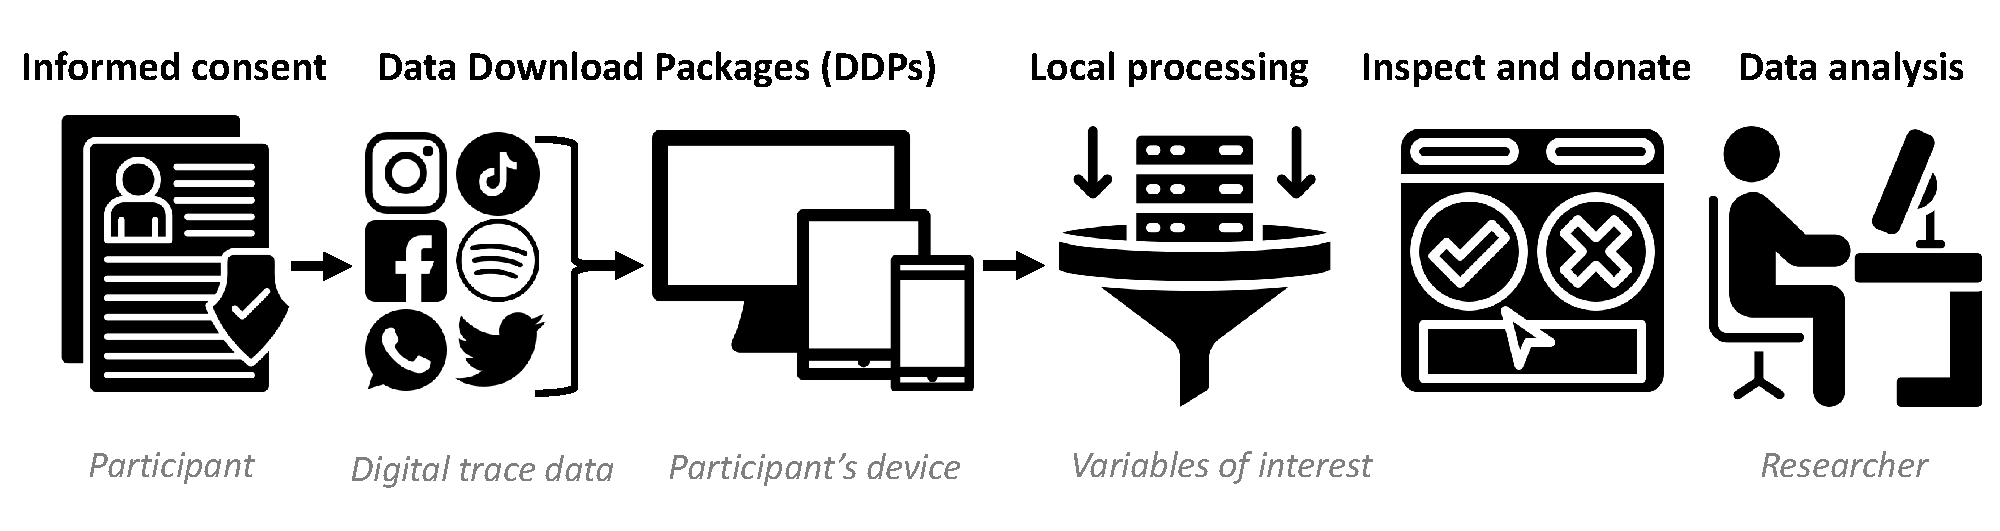
\includegraphics{data_donation_flow.pdf}
\caption{Figure 1: An overview of the participant's data donation flow
as presented by Boeschoten, Ausloos, et al. (2022).\label{fig:workflow}}
\end{figure}

In the last years, researchers have used multiple approaches to deal
with the privacy issues related to donation of DDPs. For example, van
Driel et al. (2022) requested participants to share their complete
Instagram DDPs, which were immediately de-identified prior to further
analyses (Boeschoten et al. 2021). Kmetty and Németh (2022) asked
participants to visit a research site, where participants downloaded
their DDPs which were then de-identified under the participant's
supervision. Araujo et al. (2022) developed software that allows
participants to decide per data instance within a DDP whether they want
to make it available for donation. Boeschoten, Mendrik, et al. (2022)
introduced a proof-of-concept of the software Port, allowing for local
processing of DDPs which results in aggregated, de-identified data.

In this paper, we introduce a new version of Port. It is open-source and
allows for researchers to fully configure their own data donation study.
It creates an app that guides participants through the data donation
steps. Researchers can tailor this app to the DDP of their platform of
interest and process these in their desired ways. In addition to local
processing, key features from OSD2F are also integrated, allowing
participants to decide per data instance whether they want to exclude it
from being donated. Note that researchers always ask permission from
their own Ethical Review Boards (ERBs) and Data Protections Officers
(DPOs), and that using Port does not dismiss researchers from these
obligations. The purpose of Port is to enable researchers to access
platform user data with a GDPR compliant approach.

\hypertarget{which-digital-platforms-are-investigated}{%
\section{Which digital platforms are
investigated?}\label{which-digital-platforms-are-investigated}}

Port is a tool that allows researchers to collect digital traces through
donation of DDPs. In practice, this means that Port can be configured to
process DDPs from any data controller. i.e, any legal entity that
processes personal data. However, collection of digital traces through
data donation using Port can only be a viable approach for data
collection if the platform acting as data controller meets certain
criteria.

First, in order for data donation research to occur, a platform must
comply with the individual data access request that was submitted to it,
meaning that platform compliance with the GDPR is a condition sine qua
non for effective data donation research. Second, the process to request
a copy of one's personal data should be standardized to a certain extent
such that researchers can provide study participants with instructions
on how to do this. Third, the file format of the DDP should ideally have
a certain level of standardization as well. It is not possible to plan
the procedure or extraction data from the DDP if it is unknown to the
researcher where the data of interest can be found within the DDP.

\hypertarget{how-are-digital-traces-extracted}{%
\section{How are digital traces
extracted?}\label{how-are-digital-traces-extracted}}

Port consists of two distinct elements, which are both fully controlled
by a Python script that runs locally in the browser of the participant.
This Python script is specifically tailored for each data donation
study. The first element is the data donation study flow. The goal of
this part of the Python script is to provide explanations or
instructions to the participant at various steps of the flow. The second
element is the data extraction process. The goal of this part is to make
sure that only the digital traces that are of interest to the researcher
are extracted from the DDPs and that were agreed upon by the
participant.

To run a custom Python script, Port makes use of Pyodide (The Pyodide
development team 2021). Pyodide is a Python distribution for the browser
based on WebAssembly (WebAssembly 2021).

Running the custom Python script using Pyodide in the browser of a
participant works as follows:

\begin{itemize}
\tightlist
\item
  The Python script starts and begins to run synchronously, until:

  \begin{enumerate}
  \def\labelenumi{\arabic{enumi}.}
  \tightlist
  \item
    The script reaches a Python class resembling a UI element that
    should be shown on screen, a React component (React 2022).
  \item
    The script yields and communicates with the app which UI should be
    rendered on screen.
  \item
    The participant interacts with the UI element.
  \item
    The outcome of the interaction is passed back to the Python script
    and can be handled accordingly.
  \end{enumerate}
\item
  Steps 1 through 4 are repeated until the end of the Python script.
\end{itemize}

A Python script for a data donation study typically contains the
following steps:

\begin{itemize}
\tightlist
\item
  The welcome screen for the data donation process is shown.
\item
  The participant is asked to submit their DDP.
\item
  The input is validated.
\item
  The digital traces of interest to the researcher are extracted from
  the DDP.
\item
  The extracted digital traces are placed in a table.
\item
  The table is rendered on screen.
\item
  The participant clicks on the `Yes, donate' or `No' button.
\item
  The closing screen is shown.
\end{itemize}

\begin{figure}
\centering
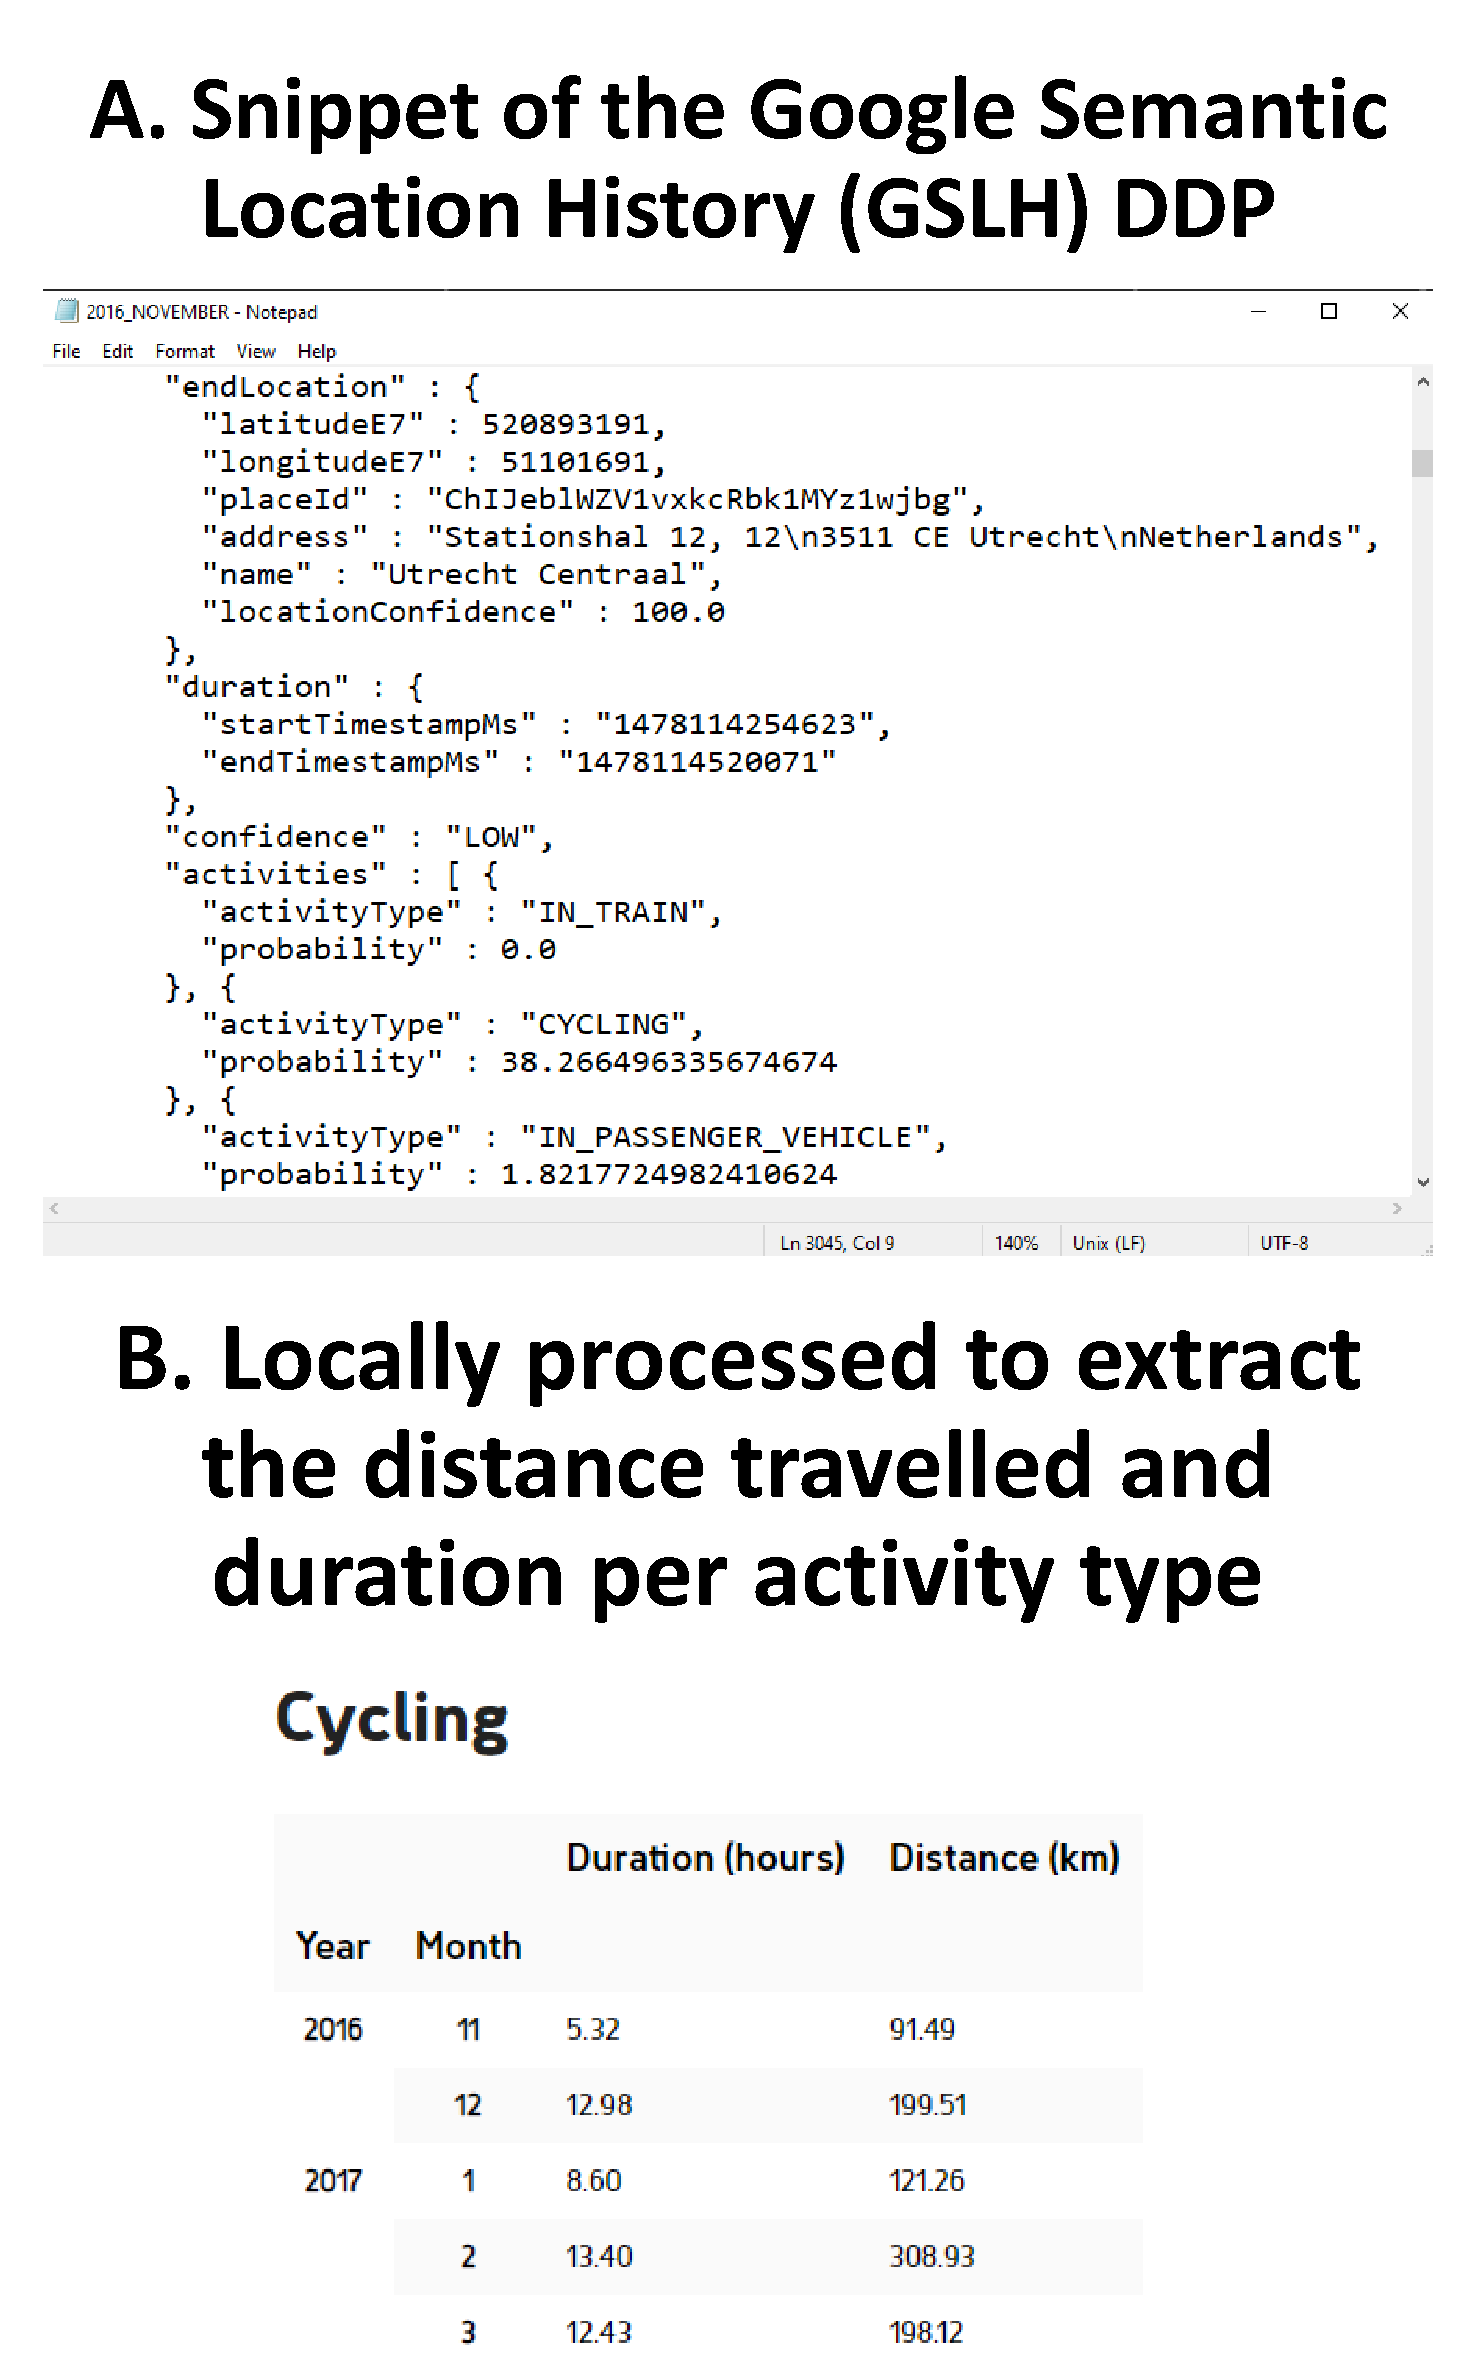
\includegraphics{GSLH_image.pdf}
\caption{A. shows an example of a location visit in the Google Semantic
Location History (GSLH) Data Download Package (DDP). B. shows how this
DDP was processed into a frequency table presenting the distance and
duration per activity type per month. \label{fig:gslh}}
\end{figure}

The benefit of having a Python script running inside the browser is that
the researcher has familiar tools to design the extraction process in
such a way that the privacy of the participants is preserved as much as
possible. For this purpose, the researcher can make use of two important
features. First, besides extracting digital traces from the DDP, it is
also possible to further process these to better match the research
question. \autoref{fig:gslh} shows an example of raw Google Semantic
Location History (GSLH) data that is locally processed to only extract
the duration and distance of the various activities tracked by GSLH per
month.

\begin{figure}
\centering
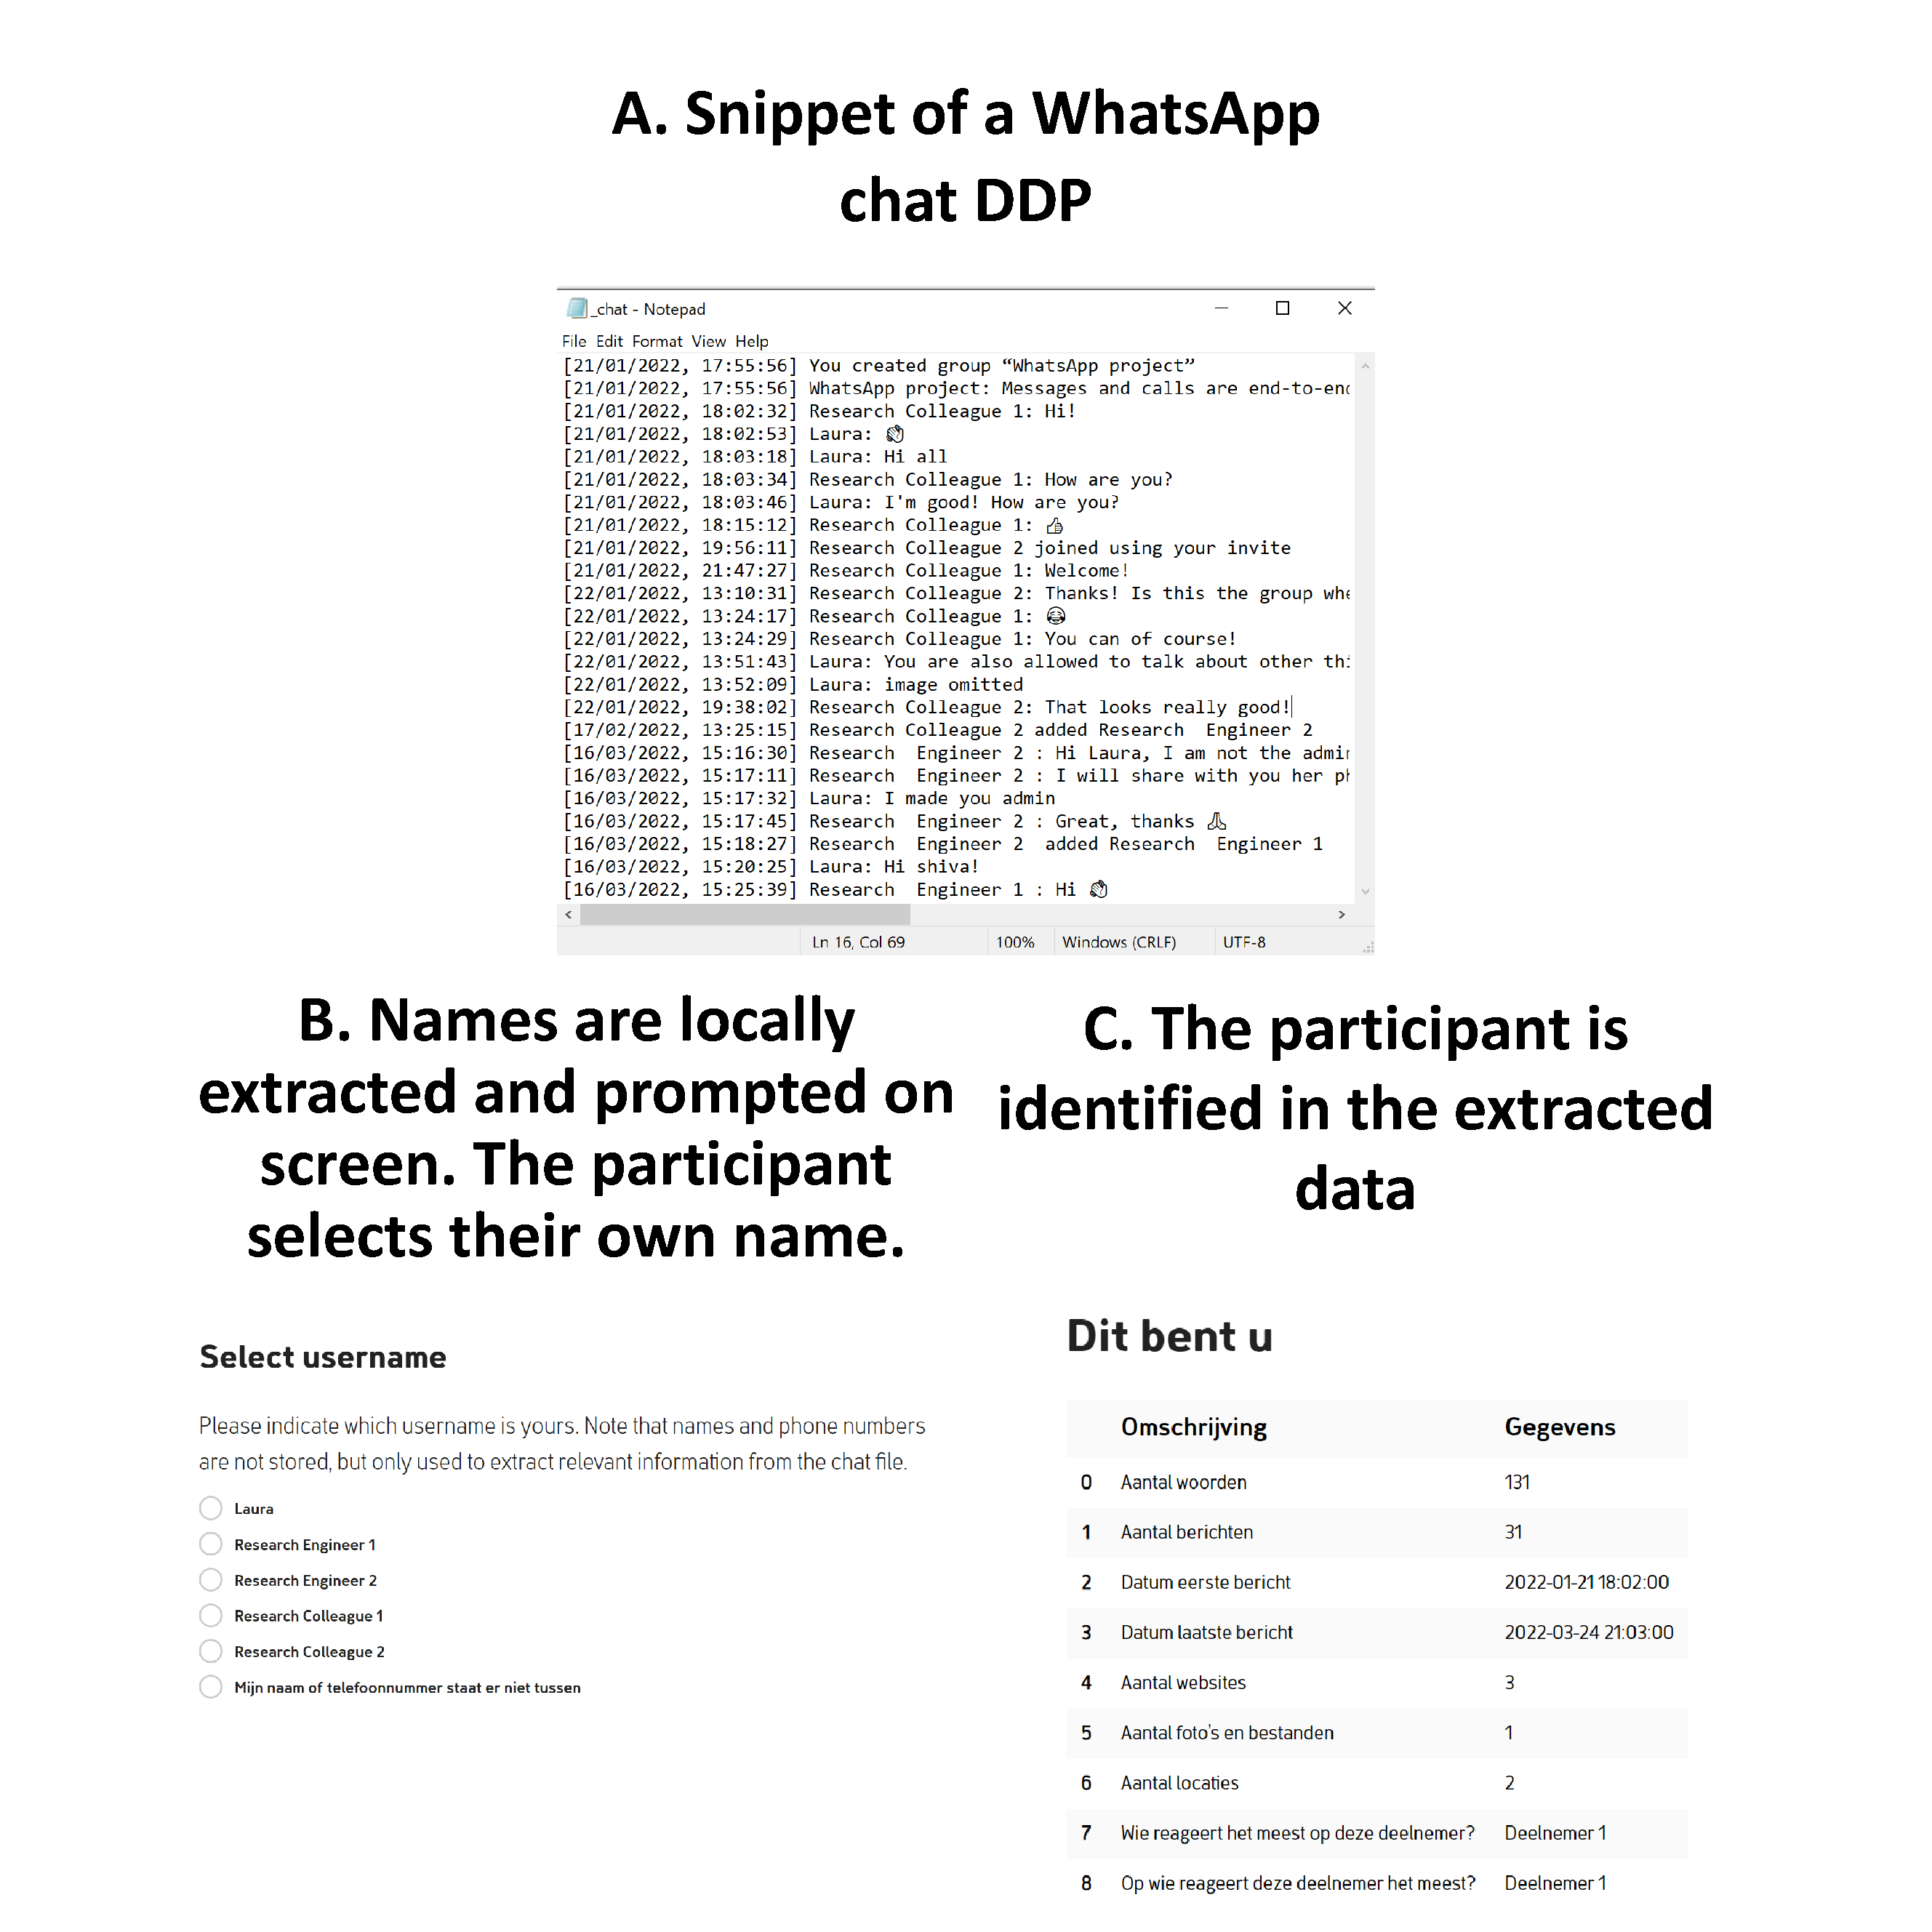
\includegraphics{WhatsApp_image.pdf}
\caption{A. shows an example of a WhatsApp chat Data Download Package
(DDP). B. shows how first only the usernames of the members in this chat
were locally extracted. The participant can select their own username
from this list. C. shows how this DDP was processed into a frequency
table presenting among other things how often the members respond to
each other's actions. Here, the participant is identified, the others
receive anonymous labels. Note that the output is presented in Dutch
\label{fig:whatsapp}}
\end{figure}

Second, a local interaction between the participant and the DDP can be
added as well, so that the participant can provide context to the data.
\autoref{fig:whatsapp} shows an example using a DDP of a WhatsApp group
chat. The Python scriptextracts the names of all people in the chat,
which are then presented to the participant in a way that they can
select their own name. This functionality can for example be used to
identify the participant within their WhatsApp group in order to extract
the messages that were written by the participant and discard all others
in the group chat, or to count the number of messages to and from the
participant. This functionality allows for the preservation of the
privacy of other people in the group chat by asking feedback from the
participant, since these people have not consented to the use of their
data.

\hypertarget{how-are-the-extracted-digital-traces-visualized}{%
\section{How are the extracted digital traces
visualized?}\label{how-are-the-extracted-digital-traces-visualized}}

\begin{figure}
\centering
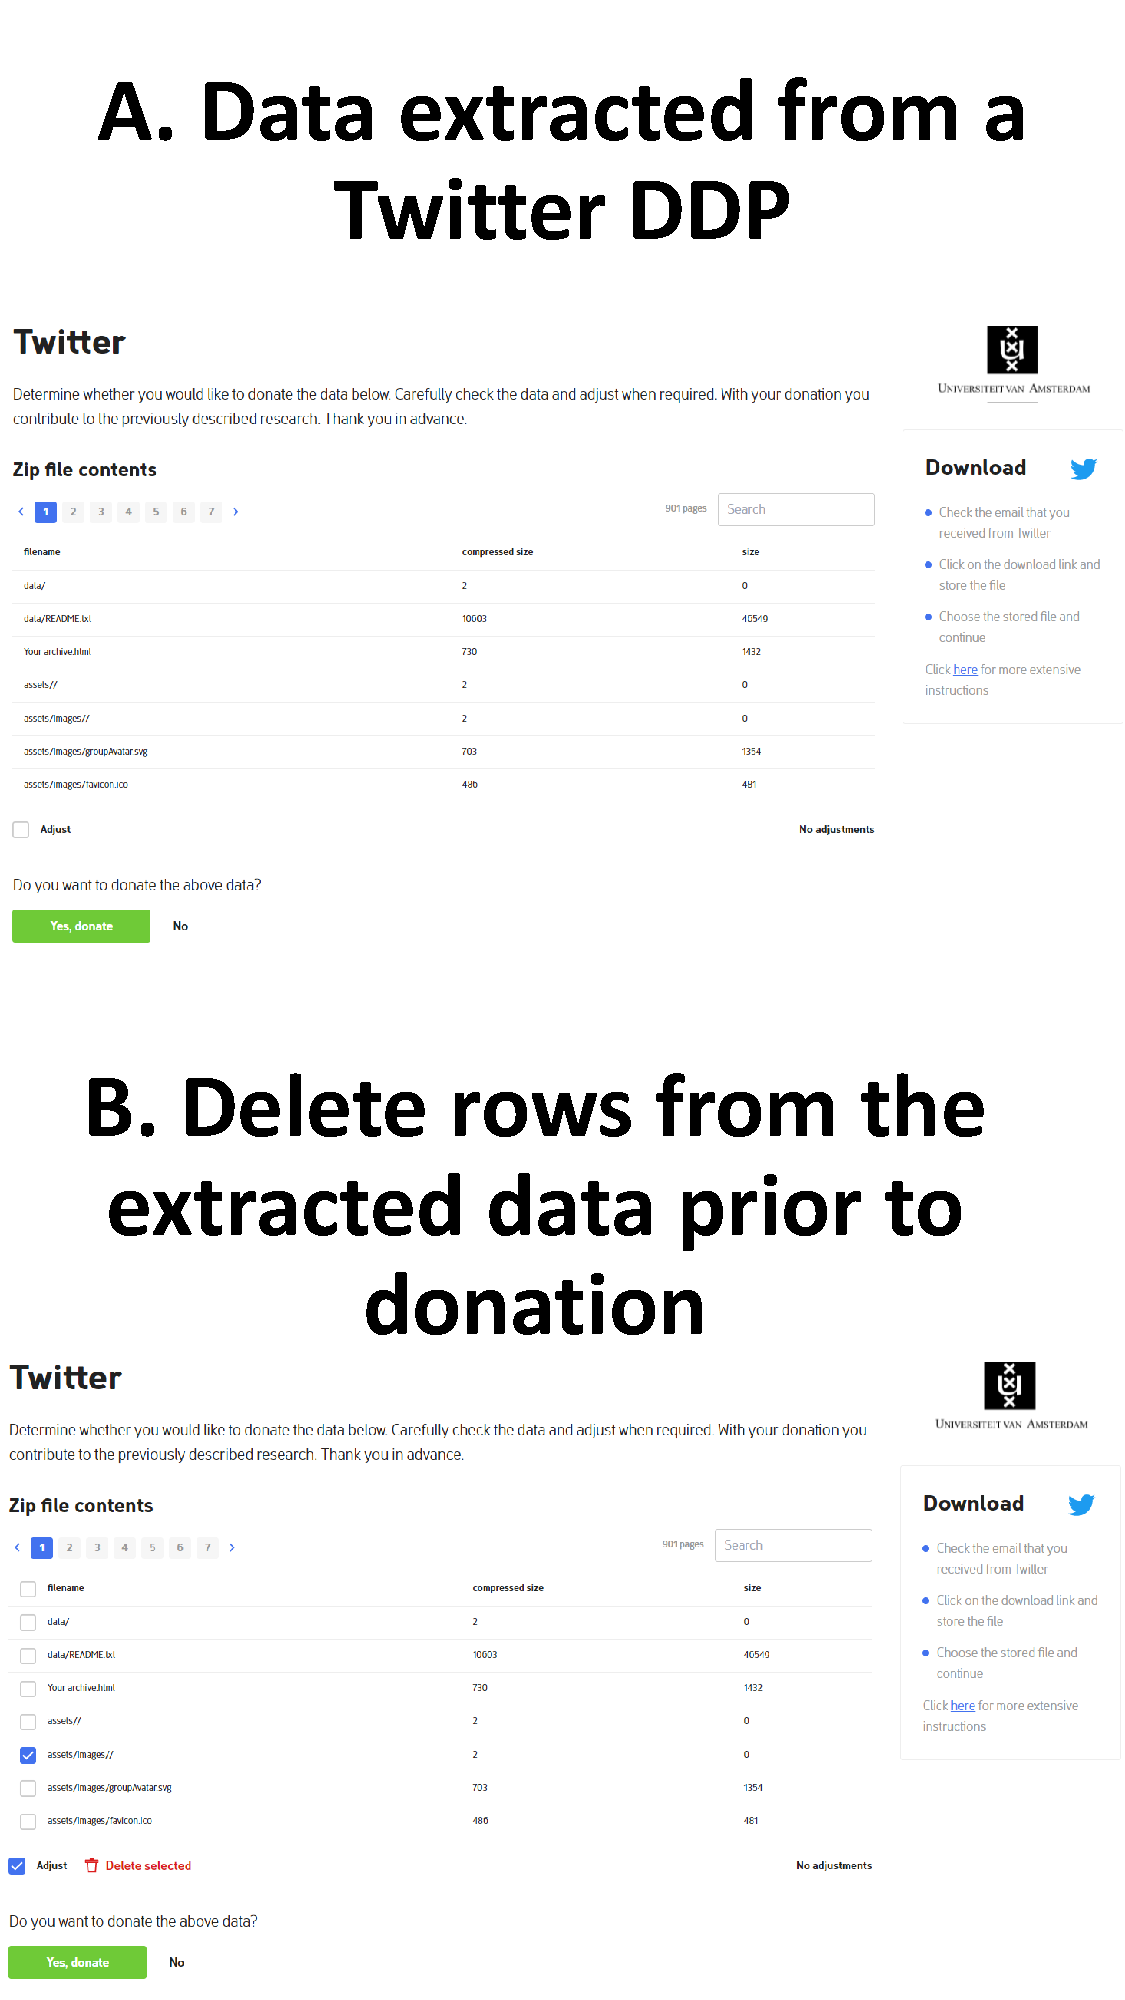
\includegraphics{Twitter_image.pdf}
\caption{The left image shows an example of data that is extracted from
a YouTube DDP, and is presented to a participant prior to providing
consent. The participant can click on the `adjust' button, after which
rows can be selected for deletion (see right image).
\label{fig:twitter}}
\end{figure}

After data extraction and potential further processing (as for example
shown in \autoref{fig:gslh}), the data is shown on screen for the
participants to review, so that they can determine whether to donate the
data. The data is shown to provide participants insight into what they
share exactly, in order for them to provide a truly informed consent
when deciding to donate this data to the researcher. This visualization
step also provides the participant with more autonomy over what is
shared, as they can select specific data instances and delete them prior
to donation (see \autoref{fig:twitter}). Providing participants with
this option is particularly interesting when working with sensitive
data, such as text messages. Researchers that receive the donated data
are informed by Port that data was deleted, but not which data was
deleted. Custom user interface elements could be developed to allow for
other types of interactions, such as labeling the data, or to present
the data in other formats, such as in histograms, if suitable.

\hypertarget{what-is-communicated-to-the-participant}{%
\section{What is communicated to the
participant?}\label{what-is-communicated-to-the-participant}}

Where a researcher invites participants for a data donation study, they
may communicate their intentions to inform the individual participants.
For example, researchers can generally inform participants in a more
generic privacy policy about the purpose of the study or about the
instructions on how to request and download the DDP of interest. Yet, to
obtain unambiguous, specific and informed consent from individual
participants, a researcher's consent form should indicate the specific
purposes of the processing for which the use of a participant's personal
data is intended. To communicate this information for a specific data
donation study, all text that is prompted on screen can be adjusted.
Currently, two languages (Dutch and English) are supported. There is
room to link to external documents, which we have used in multiple
studies to refer to the privacy policy and a document with data request
and download instructions. Finally, Port collects paradata such as time
stamps, information on clicks and navigation during the donation
process. This paradata can be used to monitor if the information
provided to the participants is clear or if there are problems with
particular aspects.

\hypertarget{acknowledgements}{%
\section{Acknowledgements}\label{acknowledgements}}

The development of Port was made possible by the
\href{http://www.pdi-ssh.nl}{Platform Digitale Infrastructuur SSH} in
the Netherlands (``Digital Data Donation Infrastructure (D3I)'').

\hypertarget{references}{%
\section*{References}\label{references}}
\addcontentsline{toc}{section}{References}

\hypertarget{refs}{}
\begin{CSLReferences}{1}{0}
\leavevmode\vadjust pre{\hypertarget{ref-araujo2022osd2f}{}}%
Araujo, Theo, Jef Ausloos, Wouter van Atteveldt, Felicia Loecherbach,
Judith Moeller, Jakob Ohme, Damian Trilling, Bob van de Velde, Claes De
Vreese, and Kasper Welbers. 2022. {``OSD2F: An Open-Source Data Donation
Framework.''} \emph{Computational Communication Research} 4 (2):
372--87.

\leavevmode\vadjust pre{\hypertarget{ref-ausloos2019gdpr}{}}%
Ausloos, Jef et al. 2019. {``GDPR Transparency as a Research Method.''}
\emph{SSRN Electronic Journal, May}, 1--23.

\leavevmode\vadjust pre{\hypertarget{ref-boeschoten2022framework}{}}%
Boeschoten, Laura, Jef Ausloos, Judith E Möller, Theo Araujo, and Daniel
L Oberski. 2022. {``A Framework for Privacy Preserving Digital Trace
Data Collection Through Data Donation.''} \emph{Computational
Communication Research} 4 (2): 388--423.

\leavevmode\vadjust pre{\hypertarget{ref-boeschoten2022privacy}{}}%
Boeschoten, Laura, Adriënne Mendrik, Emiel van der Veen, Jeroen
Vloothuis, Haili Hu, Roos Voorvaart, and Daniel L Oberski. 2022.
{``Privacy-Preserving Local Analysis of Digital Trace Data: A
Proof-of-Concept.''} \emph{Patterns} 3 (3): 100444.

\leavevmode\vadjust pre{\hypertarget{ref-boeschoten2021automatic}{}}%
Boeschoten, Laura, Roos Voorvaart, Ruben Van Den Goorbergh, Casper
Kaandorp, and Martine De Vos. 2021. {``Automatic de-Identification of
Data Download Packages.''} \emph{Data Science} 4 (2): 101--20.

\leavevmode\vadjust pre{\hypertarget{ref-bruns2019after}{}}%
Bruns, Axel. 2019. {``After the {`APIcalypse'}: Social Media Platforms
and Their Fight Against Critical Scholarly Research.''}
\emph{Information, Communication \& Society} 22 (11): 1544--66.

\leavevmode\vadjust pre{\hypertarget{ref-freelon2018computational}{}}%
Freelon, Deen. 2018. {``Computational Research in the Post-API Age.''}
\emph{Political Communication} 35 (4): 665--68.

\leavevmode\vadjust pre{\hypertarget{ref-king2011ensuring}{}}%
King, Gary. 2011. {``Ensuring the Data-Rich Future of the Social
Sciences.''} \emph{Science} 331 (6018): 719--21.

\leavevmode\vadjust pre{\hypertarget{ref-king2020new}{}}%
King, Gary, and Nathaniel Persily. 2020. {``A New Model for
Industry--Academic Partnerships.''} \emph{PS: Political Science \&
Politics} 53 (4): 703--9.

\leavevmode\vadjust pre{\hypertarget{ref-kmetty2022your}{}}%
Kmetty, Zoltán, and Renáta Németh. 2022. {``Which Is Your Favorite Music
Genre? A Validity Comparison of Facebook Data and Survey Data.''}
\emph{Bulletin of Sociological Methodology/Bulletin de M{é}thodologie
Sociologique} 154 (1): 82--104.

\leavevmode\vadjust pre{\hypertarget{ref-perriam2020digital}{}}%
Perriam, Jessamy, Andreas Birkbak, and Andy Freeman. 2020. {``Digital
Methods in a Post-API Environment.''} \emph{International Journal of
Social Research Methodology} 23 (3): 277--90.

\leavevmode\vadjust pre{\hypertarget{ref-React}{}}%
React. 2022. {``React.''} \emph{React}. \url{https://react.dev/}.

\leavevmode\vadjust pre{\hypertarget{ref-pyodide_2021}{}}%
The Pyodide development team. 2021. \emph{Pyodide/Pyodide} (version
0.23.0). Zenodo. \url{https://doi.org/10.5281/zenodo.5156931}.

\leavevmode\vadjust pre{\hypertarget{ref-van2022promises}{}}%
van Driel, Irene I, Anastasia Giachanou, J Loes Pouwels, Laura
Boeschoten, Ine Beyens, and Patti M Valkenburg. 2022. {``Promises and
Pitfalls of Social Media Data Donations.''} \emph{Communication Methods
and Measures} 16 (4): 266--82.

\leavevmode\vadjust pre{\hypertarget{ref-WebAssembly}{}}%
WebAssembly. 2021. {``WebAssembly.''} \emph{WebAssembly}.
\url{https://webassembly.org/}.

\end{CSLReferences}

\end{document}
